\documentclass[xcolor=dvipsnames]{beamer}
\usepackage[utf8]{inputenc}
\usepackage{hyperref}
\usepackage[super]{nth} % for 1st, 2nd, etc...
\setbeamertemplate{caption}[numbered] %for figures numbering

\usetheme{CambridgeUS}

\definecolor{UBCblue}{rgb}{0.04706, 0.13725, 0.26667} % UBC Blue (primary)
\definecolor{UBCgrey}{rgb}{0, 0.46, 0.7} % UBC Grey (secondary)

\setbeamercolor{title}{bg=UBCblue,fg=white}
\setbeamercolor{frametitle}{bg=UBCblue, fg=white}
\setbeamercolor{palette primary}{bg=UBCblue,fg=white} %basso a destra
\setbeamercolor{palette secondary}{fg=UBCblue} %basso al centro
\setbeamercolor{palette tertiary}{bg=UBCgrey,fg=white} %basso e alto a sx 

\setbeamercolor{structure}{fg=UBCblue} % itemize, enumerate, etc
\setbeamercolor{section in toc}{fg=UBCblue} % TOC sections
\setbeamercolor{block title}{bg=UBCgrey!50,fg=black}

%------------------------------------------------------------
%This block of code defines the information to appear in the
%Title page
\title[Emotion Patterns in Music Playlists] %optional
{Emotion Patterns in Music Playlists}

%\subtitle{\nth{1} meeting}

\author[Sara, Mario] % (optional)
{Sara Giammusso\inst{1}\inst{2} \and Mario Guerriero \inst{1}\inst{2}}

\institute[EURECOM] % (optional)
{
 \inst{1}
 Data Science Department, EURECOM, T\'el\'ecom ParisTech, France\\
  \inst{2}%
 Department of Control and Computer Engineering, Politecnico di Torino, Italy
}


\date[2018 March 22] % (optional)
{First Project meeting}


%End of title page configuration block
%-----------------------------------------------------------



%------------------------------------------------------------
%The next block of commands puts the table of contents at the 
%beginning of each section and highlights the current section:

\AtBeginSection[]
{
  \begin{frame}
    \frametitle{Table of Contents}
    \tableofcontents[currentsection]
  \end{frame}
}
%------------------------------------------------------------


\begin{document}

%The next statement creates the title page.
\frame{\titlepage}

%---------------------------------------------------------
%This block of code is for the table of contents after
%the title page
\begin{frame}
\frametitle{Table of Contents}
\tableofcontents
\end{frame}
%---------------------------------------------------------

\section{Introduction}
%Sentiment analysis (SA)
\begin{frame}
\frametitle{Sentimental Analysis (SA)}
\begin{columns}
\column{0.5\textwidth}
\begin{definition}
Sentiment Analysis (SA) is the computational study of people's opinions, attitudes and emotions toward an entity.
\end{definition}
Entity = individuals, events or topics.
\column{0.5\textwidth}
\begin{figure}
	\centering
	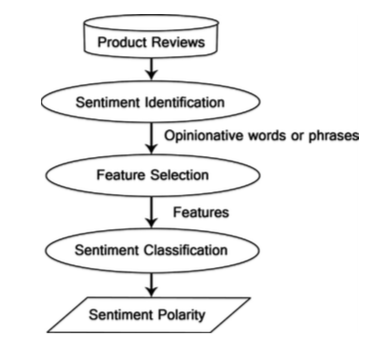
\includegraphics[scale=0.45]{./images/sa_process}
	\caption{Sentiment analysis process on product reviews}
\end{figure}
\end{columns}
\end{frame}

%Sentiment analysis: a classification problem
\begin{frame}
\frametitle{Sentiment analysis: a classification problem}
\begin{figure}
	\centering
	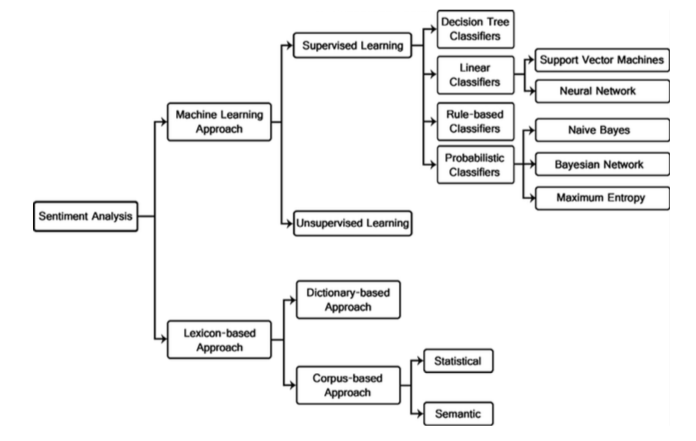
\includegraphics[scale=0.4]{./images/sentiment_classification}
	\caption{Sentiment classification techniques}
\end{figure}
\end{frame}

%Emotion Detection (ED)
\begin{frame}
\frametitle{Emotion Detection (ED)}
\begin{definition}
Emotion detection is the process of identifying human emotions.
\end{definition}
\begin{block}{Remark}
Emotion Detection (ED) is a SA task.
\end{block}
SA: detects positive or negative feeling from text.\\
ED: detects various emotions.\\
As a SA task, ED can be implemented using:
\begin{itemize}
\item ML approach
\item Lexicon-based approach
\end{itemize}
\end{frame}

%Emotion Detection: Why
\begin{frame}
\frametitle{Emotion Detection: Why}
Emotion detection has useful applications, such as: 
\begin{itemize}
\item Measure citizens happiness
\item Pervasive computing
\item Understanding the consumer
\end{itemize}
\begin{block}{Our goal}
Unravel emotion patterns in the playlists
\end{block}
\end{frame}

%Emotion Detection: Challenges
\begin{frame}
\frametitle{Emotion Detection: Challenges}
(Some of the) Biggest challenges in ED:
\begin{itemize}
\item Context-dependence of emotions $\Rightarrow $ people use different emotion regulation strategies in different social contexts
\item Word-sense disambiguation $\Rightarrow $ identifying which sense of a word (i.e. meaning) is used in a sentence, when the word has multiple meanings
\item Co-reference resolution $\Rightarrow $ pronouns and other referring expressions must be connected to the right individuals
\item Lack of labelled emotion database
\end{itemize}
\end{frame}

\section{The task}
% Feature selection
\begin{frame}{Feature Selection}
Which textual features are we interested in?
\begin{itemize}
\item Terms presence and frequency
\item Adjective
\item Opinion Words and Phrases
\item Negation expressions
\end{itemize}
\end{frame}

% Feature selection methods
\begin{frame}{Feature Selection Methods}
\begin{itemize}
\item Strings
\begin{itemize}
\item Phrases representing emotional patterns
\end{itemize}
\item Bag of Words (BoW)
\begin{itemize}
\item Sort of keywords list
\item Make the classification process simpler
\end{itemize}
\end{itemize}
\end{frame}

% Classification Levels I
\begin{frame}{Classification Levels (I)}
Three possible classification levels:
\begin{itemize}
\item Document Level 
\begin{itemize}
\item The whole document is the classification unit
\end{itemize}
\item Sentence Level
\begin{itemize}
\item Sentences are the basic classification units
\end{itemize}
\item Aspect Level
\begin{itemize}
\item Classify sentiments with respect to entities and their aspects
\end{itemize}
\end{itemize}
\end{frame}

% Classification Levels II
\begin{frame}{Classification Levels (II)}
\textbf{Document level} classification suits our problem
\begin{itemize}
\item We will analyze lyrics
\item Lyrics are (usually) small documents focused on a single topic
\item We can treat lyrics as our classification unit
\end{itemize}
\end{frame}

\section{State of the art}

%References

\section{References}
\begin{frame}{References}
\setbeamertemplate{bibliography item}[triangle]
 \begin{thebibliography}{99} % Beamer does not support BibTeX so references must be nserted manually as below
\bibitem[Microsoft, 2015]{p1} Microsoft Developer Blog (2015)
\newblock Emotion detection and recognition from text using Deep Learning
\newblock \href{https://www.microsoft.com/developerblog/2015/11/29/emotion-detection-and-recognition-from-text-using-deep-learning/}{link}

\bibitem[Survey 2014]{p2} Walaa Medhat, Ahmed Hassan, and Hoda Korashy (2014)
\newblock Sentiment Analysis Algorithms and Applications: A Survey.
\newblock \emph{Ain Shams Engineering Journal}

\end{thebibliography}

\end{frame}
%---------------------------------------------------------

\end{document}
